\documentclass[aspectratio=169]{beamer}
\usetheme{Madrid} %tema do slide. Tem muitos temas existentes... Gosto desse! Se vcs quiserem mais temas, visitem: http://deic.uab.es/~iblanes/beamer_gallery/index_by_theme.html
\usepackage[brazil]{babel} %texto
\usepackage[utf8]{inputenc} %texto
\usepackage{graphicx} %imagem	
\usepackage{caption} %imagem
\usepackage{subcaption} %imagem
\usepackage{float} %imagem e tabelas
\usepackage{booktabs} %tabelas	
\usepackage[abnt-emphasize=bf,alf]{abntex2cite} %citacoes ABNT
\usepackage{booktabs}
\graphicspath{{./Figuras/}} %Colarimages na pasta "Figuras". Gosto de fazer isso para organizar os arquivos.
\usepackage[ruled, linesnumbered]{algorithm2e}  
\usepackage[utf8]{inputenc}
\DeclareUnicodeCharacter{2009}{-}% support older LaTeX versions  		

\begin{document}
	% EDITAR ESSAS INFORMACOES (INICIO)
	\title[Projeto e Análise de Algoritmo]{Algoritmo Merge-Sort}
	\author[PPGMCS]{DANILA MARRIEL BAETA NASCIMENTO\\
		GLAYSON PARAISO MACEDO	\\
		JHEAN MARCEL SOARES COSTA\\	
		JONATAS LEITE SOUZA	\\
		LEONARDO VIEIRA GUIMARÃES\\	
		MATHEUS SILVEIRA BORGES\\	
		NARA MIRANDA DE OLIVEIRA CANGUSSU}
	\institute[]{UNIMONTES}
	\date[2017]{19 de Julho de 2017}
	% EDITAR ESSAS INFORMACOES (FIM)
	
	\begin{frame}
		\titlepage
	\end{frame}
	\begin{frame}
		\frametitle{Sum\'{a}rio}
		\tableofcontents%[pausesections]
	\end{frame}
	
%---------------------------------------------------------------------------
	% PRIMEIRA SECAO
	\section{Introdução e Contextualização}
%---------------------------------------------------------------------------

	% SLIDE 1	
	\begin{frame}
		\frametitle{Introdução}		
		\framesubtitle{Algoritmos de Ordenação}		
		\begin{itemize}
			\item A ordenação de dados é uma das funções mais utilizadas no desenvolvimento de programas de computador.
			\item Para tal, estão disponíveis na literatura inúmeros algoritmos de ordenação, com diferentes estratégias e complexidades. 
			\item Encontrar o melhor entre eles depende de algumas condicionantes, como por exemplo o tamanho de entrada.
		\end{itemize}
	
		
	\end{frame}
	% SLIDE 	
	\begin{frame}
	 	Cormen (2015) e Cormem \textit{et al} (2002) relatam  os seguintes Algoritmos de Ordenação:
	 	\begin{itemize}
	 		\item Inserção ou Insertion-Sort
	 		\item Seleção ou Selection-Sort
	 		\item Intercalação ou Merge-Sort
	 		\item Quick-Sort
	 		\item Bubble-Sort
	 	\end{itemize}
	\end{frame}


	% SLIDE 	
	\begin{frame}
	\frametitle{Objetivos}
	%\framesubtitle{}
	Este seminário tem como objetivo geral apresentar o algoritmo de intercalação Merge-Sort. \\
	\vspace{0.5cm}
	Também são objetivos específicos deste trabalho:
	\begin{itemize}
		\item Apresentar a estratégia Divisão e Conquista.
		\item Apresentar o funcionamento do algoritmo Merge-Sort pela ótica da recursividade;
		\item Comprovar analiticamente a complexidade deste algoritmo;
	\end{itemize}
	\end{frame}

	% SEÇÃO	
	\section{O Algoritmo Merge-Sort}
	
		% SLIDE 	
	\begin{frame}
		\frametitle{O Algoritmo Merge-Sort}
		\framesubtitle{Apresentação | Divisão e Conquista}
		\begin{itemize}
			\item O algoritmo Merge-Sort foi desenvolvido pelo matemático John Von Neumann em 1945;
			\item O algoritmo utiliza a estratégia "\textbf{dividir para conquistar}" como metodologia fundamental para solução do problema de ordenação;
			\item Na abordagem \textbf{divisão e conquista}, em um primeiro momento, o problema de desmembrado ao meio até não ser mais possível sua divisão.
			\item Em um segundo momento, as soluções dos subproblemas são mescladas entre si, gerando a solução do problema original.
		\end{itemize}	
	\end{frame}

	\begin{frame}
	\frametitle{O Algoritmo Merge-Sort}
	\framesubtitle{Divisão e Conquista}
		\begin{figure}
		\centering
		\caption{Estratégia de Divisão e Conquista.}
		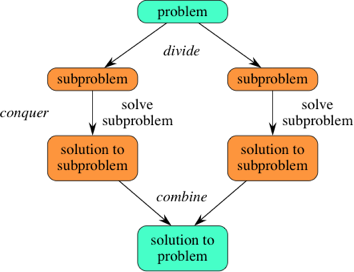
\includegraphics[width=.4\linewidth]{conquest.png}\\
		\footnotesize{Fonte: Khan Academy.}
		\label{conquest}
	\end{figure}
	\end{frame}

	\begin{frame}
	\begin{itemize}
		\frametitle{O Algoritmo Merge-Sort}
		\framesubtitle{Divisão e Conquista}
		\item Segundo Cormem (2015), a divisão repetitiva do tamanho do subvetor ao meio dá origem a ideia de tempo de execução igual à O(lg n) para o Algoritmo Merge-Sort, o que iremos provar mais adiante.
		\item No caso do algoritmo de ordenação, na primeira estapa, os elementos a serem ordenados (nosso problema) são divididos até não ser mais possível.
		\item Em um segundo momento, os menores elementos de cada subvetores são comparados entre si, gerando um novo grupo já ordenado até. Isso ocorre até que todos os subvetores, ao fim, sejam unidos novamente em um só vetor, já ordenado.
		
	\end{itemize}
\end{frame}

	% SLIDE
\begin{frame}
	\frametitle{O Algoritmo Merge-Sort}
	\framesubtitle{Entendendo seu funcionamento}
	\begin{figure}
		\centering
		\caption{Demonstração das duas etapas que constituem a estratégia de\textbf{ Divisão e Conquista}.}
		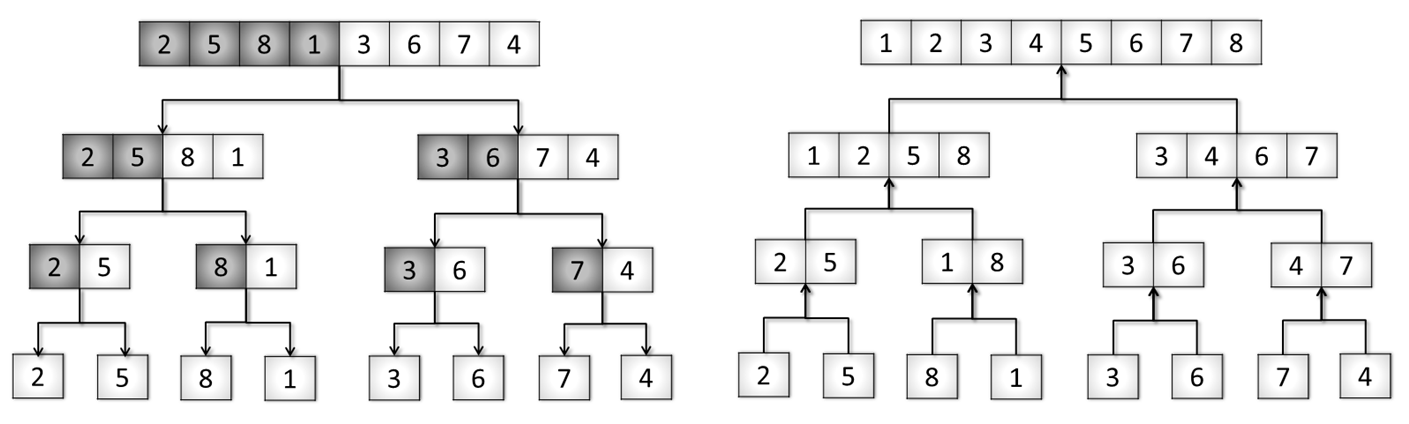
\includegraphics[width=1\linewidth]{merge2.png}\\
		\footnotesize{Fonte: Stack Overflow. Adaptado pelos Autores.}
		\label{figtextimg}
	\end{figure} 
\end{frame}



	% SLIDE 	
	\begin{frame}
	\frametitle{O Algoritmo Merge-Sort}
	\framesubtitle{Pseudocódigo}
	
	\scalebox{.6}{
		\hspace{1cm}  
		\begin{algorithm}[H]
			$ n_{1} $ = q - p + 1\\
			$ n_{2} $ = r - q\\
			\For{i crescendo de p até q}
				{B[i] = A[i]}
			\For{j crescendo de q + 1  até  r}
				{B[r+q+1-j] = A[j]}
			i = p\\
			j = r\\
			\For{k crescendo de p  até  r}
				{\eIf{B[i] <= B[j]}
					{A[k] = B[i]\\i = i + 1}
					{A[k] = B[j]\\j = j - 1}}
			\caption{\textsc{Merge-Sort}(A, p, q, r)}
			\label{alg1}
		\end{algorithm}
		}
	\end{frame}

	% SEGUNDA SECAO
\section{Recursividade e Recorrência}

	% SLIDE
\begin{frame}
	\frametitle{Recursividade e Recorrência}
	\framesubtitle{Entendendo seu funcionamento}
	\begin{itemize}
		\item O funcionamento do Merge-Sort se dá pela metodologia recursiva, onde a função é chamada por ela mesma até que o critério de parada seja satisfeito.
		\item Neste método, todas as chamadas são feitas (ocupando espaços adicionais de memória) até que a resposta inicialmente solicitada seja finalmente apresentada.
		\item No nosso algoritmo, por exemplo, antes que seja apresentado o vetor ordenado, ele irá se subdividir e posteriormente se combinar de forma já ordenada $ \lg(n) $ vezes.
	\end{itemize}
\end{frame}

	% SLIDE
	\begin{frame}
	\frametitle{Recursividade e Recorrência}
	\framesubtitle{Entendendo seu funcionamento}
	\begin{figure}
		\centering
		\caption{Análise da árvore de recursividade.}
		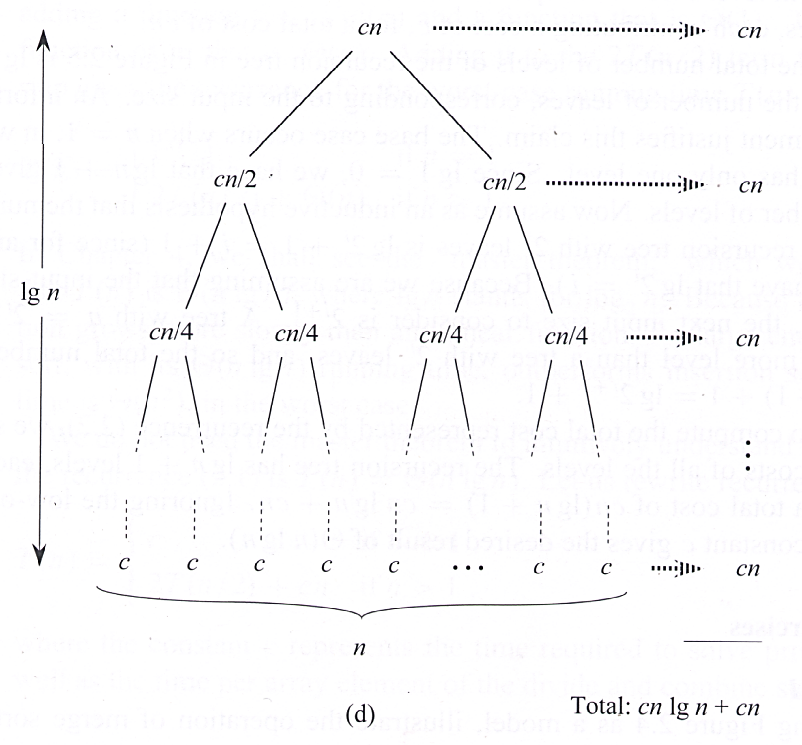
\includegraphics[width=.37\linewidth]{quickbest.png}\\
		\footnotesize{Fonte: Cormem (2002)}
		\label{figtextimg}
	\end{figure} 
	\end{frame}
	


%---------------------------------------------------------------------------
	% SEGUNDA SECAO
	\section{Análise de Complexidade}	
%---------------------------------------------------------------------------
	% SLIDE 5 - UMA TABELA	
	
	% SLIDE 	
\begin{frame}
	\frametitle{Análise de Complexidade}
	\framesubtitle{Análise do Consumo de Tempo do Algoritmo Merge-Sort}
	A análise do consumo de tempo do algoritmo Merge-Sort pode ser feita da seguinte forma:
	\vspace{1cm}
	\begin{minipage}[c]{0.49\linewidth}
		\vspace{0.7cm}
	\scalebox{.7}{
		
		\hspace{5cm}
	\begin{algorithm}[H]
		\If{p $ < $ r}
			{q = [(p+r)/2]\\
			\textsc{Merge-Sort} (A, p, q)\\
			\textsc{Merge-Sort} (A, q+1, r)\\
			\textsc{Merge-Sort} (A, p, q, r)}
			\caption{\textsc{Merge-Sort}(A,p,r)}
	\end{algorithm}
}
\end{minipage}
\hfill
	\scalebox{.7}{
		
	\begin{minipage}[c]{0.49\linewidth}
		\vspace{1cm}
		1\\
		1\\
		T([n/2])\\
		T([n/2])\\
		an+c
	\end{minipage}
}
\end{frame}

	% SLIDE 	
\begin{frame}
	\frametitle{Análise de Complexidade}
	\framesubtitle{Método Analítico}
	Com base na estratégia de\textbf{ divisão e conquista}, pode-se chegar a seguinte equação de recorrência (CORMEN, 2015):
	\begin{equation}
	T(n) = T(n/2) + T(n/2) + n
	\end{equation}
	Que podem ser representada apenas por:
	\begin{equation}
	T(n) = 2T(n/2) + n
	\end{equation}
\end{frame}

% SLIDE 	
\begin{frame}
	\frametitle{Análise de Complexidade}
	\framesubtitle{Método Analítico}
	Simulando a execução do algoritmo, podemos considerar o valor de \textit{n} em um próximo passo como sendo \textit{n/2}:
	\begin{equation}
	T(n/2) = 2T(n/2^{2}) + (n/2)
	\end{equation}
	Com T(n/2) encontrado, o substituiremos na equação (2):
	\begin{equation}
	T(n) = 2[2T(n/2^{2})+ (n/2))] + n
	\end{equation}
	Que pode ser representada apenas por:
	\begin{equation}
	T(n) = 2^{2}T(n/2^{2}) + 2n
	\end{equation}
\end{frame}

% SLIDE 	
\begin{frame}
	\frametitle{Análise de Complexidade}
	\framesubtitle{Método Analítico}
	Agora, iremos aplicar \textit{n/4} como sendo \textit{n} na equação (2).
	\begin{equation}
	T(n/4) = 2T(n/2^{3}) + (n/4)
	\end{equation}
	Agora que temos T(n/4), podemos aplicar na equação (5):
	\begin{equation}
	T(n) = 2[2^{2}T((n/2^{3}+ (n/4)) + (n/2)))] + n
	\end{equation}
	Que pode ser representada simplesmente por:
	\begin{equation}
	T(n) = 2^{3}T(n/2^{3}) + 3n
	\end{equation}
\end{frame}

% SLIDE 	
\begin{frame}
	\frametitle{Análise de Complexidade}
	\framesubtitle{Método Analítico}
	Aqui, já se consegue encontrar um padrão de crescimento da função:
	\begin{equation}
	T(n) = 2^{k}T(n/2^{k}) + kn
	\end{equation}
	Sabe-se também que quando a função atingir seu último passo de divisão, $(n/2^{k})$ será igual a 1, menor valor que pode ser assumido, sendo este, inclusive, o critério de parada da recursividade.
	
	Se igualarmos então $(n/2^{k})$ por 1, temos que:
	\begin{equation}
	\frac{n}{2^{k}} = 1 
	\end{equation}
	\begin{equation}
	n = 2^{k}
	\end{equation}
\end{frame}
%---------------------------------------------------------------------------
	% SLIDE
	\begin{frame}
		\frametitle{Análise de Complexidade}
		\framesubtitle{Método Analítico}
		Então teremos também que:
		\begin{equation}
		\lg n = k
		\end{equation}
		Substituindo os valores encontrados em (11) e (12) em (9), temos que:
		\begin{equation}
		T(n) = nT(1) + n\lg n
		\end{equation}
		Como sabemos que T(1) = 1, então:
		\begin{equation}
		T(n) = n + n\lg n
		\end{equation}
		Que pode ser entendido apenas por:

		\begin{center}
			\textbf{O(n.lg n)}	
		\end{center}

	\end{frame}



	% SLIDE
\begin{frame}
	\frametitle{Análise de Complexidade}
	\framesubtitle{Teorema Mestre}
	Podemos tratar o problema também com o Teorema Mestre, foco do trabalho anterior. Para tal, consideraremos que muitas das recorrências que ocorrem na análise de algoritmos de divisão e conquista têm a forma:
	\begin{equation}
	F(n) = aF\left(\dfrac{n}{b}\right) + cn^{k}
	\end{equation}
	\begin{theorem}
		Sejam a $ \geq $  1, b $ \geq $ 2, k $ \geq $ 0 e $ n_{0} $ $ \geq $ 1 números naturais e seja c $ > $ 0 um número real.  Seja F é uma função que leva números naturais em números reais positivos e satisfaz a recorrência para $n = n_{0}b^{1} $, $ n_{0}b^{2} $, $ n_{0}b^{3} $, 
	
	\end{theorem}
	
	
\end{frame}

\begin{frame}
	\frametitle{Análise de Complexidade}
	\framesubtitle{Teorema Mestre}
	\begin{theorem}
	Suponha que F é assintoticamente não decrescente, ou seja, que existe $ n_{1} $ tal que F(n) e F(n+1) para todo n $\geq n_{1}$. Nessas condições:
\end{theorem}
	
	\begin{itemize}
		\item Se $\dfrac{\lg a}{\lg b} > k$ então F está em $\theta$(n$\log$a); 
		\item Se $\dfrac{\lg a}{\lg b} = k$ então F está em $\theta$(nk$\log$n);
		\item Se $\dfrac{\lg a}{\lg b} < k$ então F está em $\theta$(nk). 
	\end{itemize}

\end{frame}

\begin{frame}
	\frametitle{Análise de Complexidade}
	\framesubtitle{Teorema Mestre}
	No caso do Merge-Sort, temos que:
	\begin{equation}
	F(n) = aF\left(\dfrac{n}{b}\right) + cn^{k}
	\end{equation}
	\begin{equation}
	= 2F\left(\dfrac{n}{2}\right) + n
	\end{equation}
	Assim a = 2, b = 2 e k = 1.\\
\end{frame}
\begin{frame}
\frametitle{Análise de Complexidade}
\framesubtitle{Teorema Mestre}
Efetuando as operações de verificação do Teorema Mestre:
\begin{equation}
\lg (a) = \lg (b) = \lg (2) = 1
\end{equation}
Assim temos que:
\begin{equation}
\dfrac{\lg a}{\lg b} = k = 1
\end{equation}
Portanto, como provado anteriormente, o algoritmo Merge-Sort pode ser entendido como:\\
\textbf{O(n.lg n)}	
\end{frame}
		

%---------------------------------------------------------------------------

	%SECAO DE CONCLUSÃO
	\section{Testes do Algoritmo em Máquina Real}
	\begin{frame}
		\frametitle{Testes do Algoritmo em Máquina Real}
		\framesubtitle{Arquitetura da Máquina}
		Foi implementado o algoritmo Merge-Sort em Python 3.6 utilizando a IDE PyCharm Community. Para executar os testes de consumo de tempo, foi utilizado uma máquina com as seguintes configurações:
		
	% Please add the following required packages to your document preamble:
	% \usepackage{booktabs}
% Please add the following required packages to your document preamble:
% \usepackage{booktabs}
% Please add the following required packages to your document preamble:
% \usepackage{booktabs}
\begin{table}[H]
	\centering
	\caption{Arquitetura de Máquina}
	\label{my-label}
	\begin{tabular}{@{}|l|l|@{}}
		\toprule
		\textbf{Parâmetro}  & \textbf{Configuração}            \\ \midrule
		Sistema Operacional & Windows 10 Pro                   \\ \midrule
		Processador         & Intel Core i7-5500U CPU 2.40 GHz \\ \midrule
		Memória RAM         & 8 GB                             \\ \bottomrule
	\end{tabular}
\end{table}

	\end{frame}

%SLIDE

	\begin{frame}
	\frametitle{Testes do Algoritmo em Máquina Real}
	\framesubtitle{Resultados}
	
	\begin{figure}
		\centering
		\caption{Gráfico de tempo de execução por número de entradas.}
		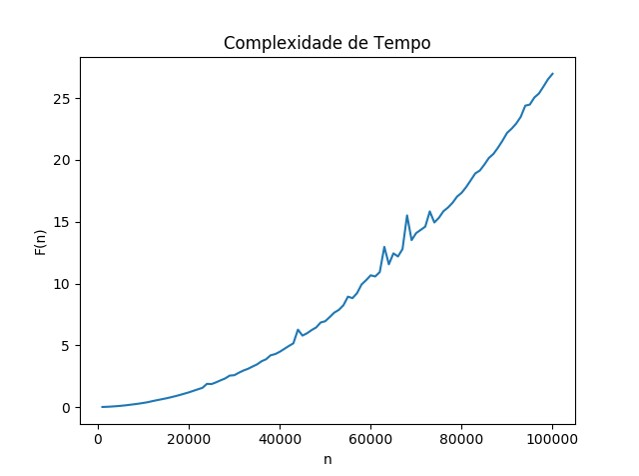
\includegraphics[width=.47\linewidth]{grafico.jpg}\\
		\footnotesize{Fonte: Os Autores}
		\label{grafico}
	\end{figure} 

	\end{frame}

	%SECAO DE CONCLUSÃO
	\section{Conclusão}
%---------------------------------------------------------------------------	
	% SLIDE  - CONCLUSÃO
	\begin{frame}
		\frametitle{Conclusão}
		\framesubtitle{Considerações Finais}
		Ao fim, pode-se chegar as seguintes considerações sobre o algoritmo tratado neste seminário:
		\begin{enumerate}
			\item O algoritmo Merge-sort faz a ordenação ocupando uma grande quantidade de memória, pelo fato de usar a estratégia de recursividade.
			\item Cormem (2014) instrui que, se a memória for um requisito de alto custo, este algoritmo não constitui uma boa escolha quando comparado com os demais algoritmos de ordenação (por inserção e seleção).
			\item Uma outra desvantagem é o fator constante, que se apresenta maior que os dos demais algoritmos. Entretanto, para grandes entradas \textit{n}, esse valor se torna desconsiderável.
		\end{enumerate}
	\end{frame}

	% SLIDE  - CONCLUSÃO
\begin{frame}
	\frametitle{Conclusão}
	\framesubtitle{Considerações Finais}
	Não obstante, pode-se listar as seguintes vantagens do algoritmo Merge-Sort:
	\begin{enumerate}

		\item O algoritmo Merge-Sort possui tempo de execução para o pior caso ($ O  n\log n $) menor do que os demais algoritmos de ordenação ($ n^{2} $), tornando-se uma excelente escolha quando o curto de memória não foi importante.
		
		\item Portanto, o algoritmo é apropriado para listas de ordenação extensas.
		
		\begin{figure}
		\centering
		\caption{Gráfico comparativo entre as funções $ n^{2}, nlog_{2} $ e $n $.}
		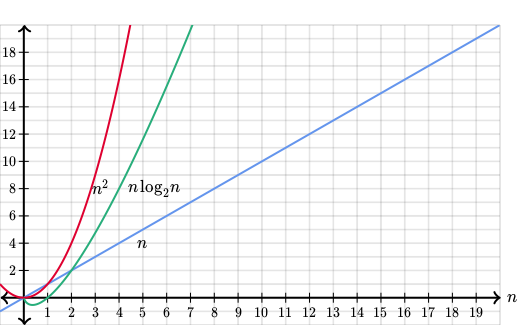
\includegraphics[width=.35\linewidth]{graficocomparativo.png}\\
		\footnotesize{Fonte: Khan Academy}
		\label{graficocomparativo}
		\end{figure} 


	\end{enumerate}
\end{frame}
%---------------------------------------------------------------------------
	%SECAO DE REFERENCIAS
	\section{Refer\^{e}ncias bibliogr\'{a}ficas}
%---------------------------------------------------------------------------
	% SLIDE  - REFERENCIAS
	\begin{frame}
		\frametitle{Refer\^{e}ncias Bibliogr\'{a}ficas}
		\begin{enumerate}
			\item CORMEN, Thomas H. et al.\textbf{ Algoritmos:} teoria e prática. Editora Campus, v. 2, 2002.
			\item CORMEN, Thomas. \textbf{Desmistificando algoritmos.} Elsevier Brasil, 2015.
		\end{enumerate}
	\end{frame}

	%---------------------------------------------------------------------------
\end{document}
